% ======================================================================
% APPENDIX (v5): the crisis check derived from the ledger, the Schur
% residue (moved here from the operator appendix), and the prototype's
% discovery check in compressed form.
% \input from changing_networked_mind_v5.tex (after the reliability appendix).
% Uses the main paper's macros (\Top, \KL, \Eq) and labels (eq:tilted,
% eq:bmr, eq:gamma, sec:structurelearning, sec:revision, tab:dials).
% ======================================================================

% ========================================================================
\section{The crisis check, the Schur residue, and the prototype's discovery check}
\label{app:crisis-discovery}
% ========================================================================

This appendix derives the simulation's threshold events from the single objective the paper
already carries, so that no structural change reads as a stipulated event. The \emph{crisis
check}, step 3 of the loop in \S\ref{sec:model} and the only structural move the model of this
paper makes, is derived in full. The \emph{Schur residue} comes next: what marginalizing a
hub leaves behind, the algebra behind both the oxygen rival of Appendix~\ref{app:null} and
the discovery direction. The \emph{discovery check} belongs only to the earlier prototype of
Appendix~\ref{app:null}: the main-text model runs reduction only
(\S\ref{sec:structurelearning}). It is derived in compressed form so the prototype's flagged
numbers remain auditable; whatever is not derived is named as a commitment at the
end.

\subsection{One ledger for every structural move}

The bounded agent of \S\ref{sec:revision} revises its beliefs by minimizing
$\KL{q}{p(x\mid o,G)}-\lambda\,\Eq{q}{U^{\!\top}\!x}$ (Eq.~\ref{eq:tilted}): fidelity to the
honest posterior, traded against the value of where the commitments land, at temperature
$\lambda$. A structural move, whether pruning an edge or waking a node, changes both terms, so
the same objective scores the move:
\begin{equation}
\mathrm{score}(M\!\to\!\tilde M)
\;=\;
\underbrace{\Delta F}_{\text{log Bayes factor}}
\;+\;
\underbrace{\Delta G}_{\text{epistemic gain}}
\;+\;
\lambda\,\underbrace{\Delta U}_{\text{conviction value}},
\qquad
\text{accept}\iff \mathrm{score}>0,
\label{eq:ledger}
\end{equation}
with $\Delta F$ the evidence for the edited structure, $\Delta G$ the expected information gain
about any newly introduced latent, which is zero for a prune, and
$\Delta U = \Eq{q_{\tilde M}}{U^{\!\top}\!x}-\Eq{q_{M}}{U^{\!\top}\!x}$ the change in the
conviction-field value of the commitments. Equation~\eqref{eq:ledger} is not a new mechanism:
it is Eq.~\eqref{eq:tilted} evaluated at two structures and differenced. Both threshold events
below are instances of it.

\subsection{The crisis check is the ledger on a prune}

For a prune, every term of Eq.~\eqref{eq:ledger} is closed-form in the linear-Gaussian setting.
The evidence half is Bayesian model reduction (Eq.~\ref{eq:bmr}): writing the agent's
accumulated likelihood deposit as $J=\Pi-\Pi_0$, $j=h-h_0$, the Savage--Dickey identity scores
the swap of the prior $(\Pi_0,h_0)$ for the edge-$e$-reduced prior $(\Pi_0^{(e)},h_0^{(e)})$
under the same likelihood, and it already exhibits the reduced posterior, a step the main text
does not spell out,
\begin{equation}
\Pi^{(e)} = \Pi_0^{(e)} + J,
\qquad
h^{(e)} = h_0^{(e)} + j ,
\end{equation}
so the value half costs one linear solve per candidate edge:
\begin{equation}
\Delta U_e \;=\; U^{\!\top}\!\bigl(\mu^{(e)}-\mu\bigr),
\qquad
\mu^{(e)} = \bigl(\Pi^{(e)}\bigr)^{-1}h^{(e)},\quad \mu = \Pi^{-1}h,
\label{eq:dU-prune}
\end{equation}
with $U=\Top u$ the agent's \emph{current} conviction field, read along its present couplings.
The crisis check is then exactly the ledger: edge $e$ is flagged iff
$\Delta F_e + \lambda\,\Delta U_e > 0$, and \emph{crisis} is the round at which both protective
belt edges are flagged, upon which the agent adopts the reduced prior composed over every edge
its own ledger flags, releasing the hub. Pruning a conviction-protective edge moves the
posterior mean away from the cherished commitments, so $\Delta U_e<0$ and the rule reproduces
the intuitive form ``the evidence must overcome $\lambda$ times the value the edge protects.''

A natural surrogate suggests itself here: the static threshold $\Delta F_e > \lambda\,v_e$ with
$v_e = |U_{\mathrm{parent}}|+|U_{\mathrm{child}}|$, the summed conviction magnitude at the
edge's endpoints, available without a solve, and with the
right \emph{form}, since it is Eq.~\eqref{eq:ledger} with $\Delta U_e \equiv -v_e$. But it has
the wrong \emph{content}: $v_e$ is a static stand-in for a quantity the model can compute exactly,
so we compute it. The difference is not cosmetic, and its direction is itself informative:
because the reduced and full posteriors share the likelihood deposit, the mean displacement of
a prune, and with it $\lambda\,\Delta U_e$, shrinks as evidence accumulates. A
data-rich paradigm is barely protected at the threshold; almost all of its persistence must
come from upstream, from the conviction gate that decides which evidence is allowed to
accumulate at all (the $\gamma$ gate, \S\ref{sec:revision}). The static surrogate would quietly overstate threshold
protection; the exact ledger locates lock-in where the paper's results put it: gating plus
isolation, not a high bar at the moment of decision.

\subsection{The Schur residue: what marginalizing a hub leaves behind}

Marginalizing a hub condenses its influence into new edges among its neighbours: for a
common-cause structure over $(x_1,x_2,b)$,
\begin{equation}
\Pi=\begin{pmatrix}2&0&1\\0&2&1\\1&1&2\end{pmatrix}
\ \xrightarrow{\ \text{marginalize } b\ }\
\begin{pmatrix}2&0\\0&2\end{pmatrix}-\tfrac12\begin{pmatrix}1\\1\end{pmatrix}\begin{pmatrix}1&1\end{pmatrix}
=\begin{pmatrix}1.5&-0.5\\-0.5&1.5\end{pmatrix},
\label{eq:schur}
\end{equation}
a direct coupling induced where the joint had a zero. Conditioning on a shared \emph{effect} is the
dual operation: two commitments that jointly feed one observation are a priori independent, and
clamping that observation anti-couples them: explaining away, run on the precision matrix. Both
operations fill in the off-diagonal coupling the carry-over cost $\kappa=\Top\bone$ is built
from, and Fig.~\ref{fig:schur-generic} draws both on the smallest nets that exhibit them.

Two of the paper's objects are instances of this residue. The oxygen rival of
Appendix~\ref{app:null} keeps exactly the direct mass-law couplings that marginalizing the
phlogiston hub leaves behind: the incumbent's Schur complement over its hub, means
corrected. Read in reverse, the residue is a \emph{signature}: a hidden hub $b$ with
couplings $c$ leaves, on marginalization, the rank-one footprint $-cc^{\!\top}/\Pi_{bb}$ in
the visible precision: exactly what the prototype's discovery check reads off the residual
below.

\begin{figure}[h!]
\centering
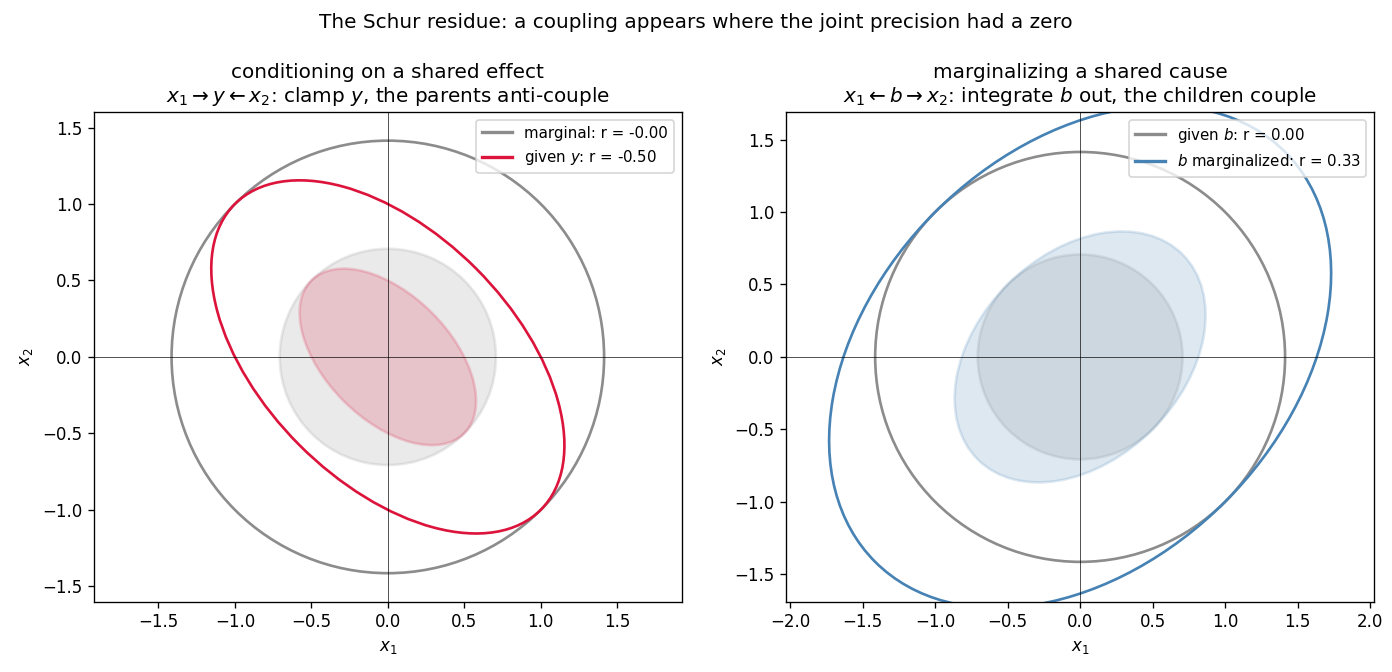
\includegraphics[width=0.60\linewidth]{fig_schur_generic.png}
\caption{The Schur residue, computed on the smallest nets that show it. Left: conditioning
on a shared effect ($x_1\!\to\!y\!\leftarrow\!x_2$): the parents are a priori independent (grey,
$r=0$); clamping their common descendant $y$ manufactures an anti-correlation (crimson,
$r=-0.50$): explaining away. Right: marginalizing a shared cause (the matrix of
Eq.~\ref{eq:schur}): the children are independent given $b$ (grey); integrating $b$ out leaves
them coupled (blue, $r=+0.33$). In both cases a coupling appears where the joint precision had a
zero: the off-diagonal mass the carry-over cost $\kappa=\Top\bone$ is built from.}
\label{fig:schur-generic}
\end{figure}

\subsection{The discovery check is the ledger on an expansion (prototype only)}

This check runs only in the earlier phlogiston prototype of Appendix~\ref{app:null}; the
model of the main text runs reduction only (\S\ref{sec:structurelearning}). Expansion cannot
be closed-form: a new node needs a real inversion, and, per Stanford's problem of unconceived
alternatives, the agent cannot plan toward a dimension it has not conceived. The check
therefore has exactly two parts, and only two:

\begin{enumerate}
\item \textbf{Arrival.} Candidate proposals arrive at a Poisson rate $r$. This is the one
place a stipulated process enters, and it is a deliberate modelling commitment: a rate is the
maximally agnostic model of conceiving what one has not conceived. The proposal's
\emph{direction} is read from the model's own prediction errors: by the rank-one footprint
above, the leading eigenvector of the windowed error second moment is the best single-hub
explanation of the residual. The window is an estimator horizon, not a gate.
\item \textbf{Acceptance.} The arrived proposal is accepted iff the model log Bayes factor of
the bordered (hub-wired) model against the agent's current one is positive: iff the residual
genuinely loads on the proposed hub. The epistemic gain $\Delta G$ sits on the other side of
the move: being positive for any new latent, it pays for attempting the
inversion, and it cannot keep a hub the data do not hold: an accept test that included it
would wake on pure noise. Entertaining is paid by curiosity; keeping is paid by evidence.
Repeated looks give the Bayes factor a small false-discovery rate, owned rather than hidden;
its principled remedy is the audited wake-then-prune cycle of Appendix~\ref{app:null}, not a
reinstated threshold.
\end{enumerate}

A tempting third part is deliberately absent: a \emph{trigger}, requiring the residual floor,
namely the eigenvalue above, to clear some height before the Bayes factor is consulted. It would
duplicate the accept test's job with a free constant, so the check has no tuned threshold:
the rate carries Stanford's commitment, the eigenvector the direction, the ledger decides.
The floor is recorded as telemetry: the visible signature of the residual the old paradigm
had been absorbing.

\subsection{What remains a modelling commitment}

The derivations leave a short list of choices not forced by the formalism; the claim that
``crisis, revolution and discovery are threshold crossings of the model's own evidence'' is
honest only with this boundary drawn:

\begin{itemize}
\item \textbf{The belt conjunction.} ``Crisis'' is operationalized as both named
mass-law edges flagged in the same round. The per-edge accept is derived; the conjunction over
those two edges is our operational definition of having eliminated the phlogiston mass-law
reading.
\item \textbf{The ordering: a result, not a commitment.} The prototype attempts expansion
only after an agent's own crisis, but the ordering is enforced by the evidence rather than by
fiat: running the identical proposal + ledger pipeline for every pre-crisis agent at every
step, without applying it, the ledger rejects $13{,}180$ of $13{,}185$ pre-crisis
agent-steps, and the five crossings are marginal ($\Delta F < 0.005$): the repeated-look
false-positive rate owned above. The intact paradigm absorbs the residual; there is nothing
for the check to find until reduction exposes it.
\item \textbf{The Poisson rate $r$} (swept), the prediction-error \emph{window} (an estimator
horizon), a short \emph{warm-up} before reduction is permitted (an initialization guard), and
the released hub's self-precision are quantitative choices of the same standing as the other
prototype dials of Table~\ref{tab:dials}.
\end{itemize}

% ========================================================================
